%!TEX root = ../report.tex

\begin{document}
    \chapter{Task 1.1}
    \section{Deliverables 1.1}
    \begin{itemize}
        \item[] Write a report detailing your envisaged experimental setup, expected problems and expected performance. In your report, use terminology from the lecture (i.e. measurement system, measurand, measured quantity, and so forth) to describe your experiment. Your report should cover:
    \end{itemize}
    
    \begin{itemize}
        \item[1.] The relevant aspects of the design of the robot, especially how you mark the stop position and how you ensure identical start positions.
        \item[2.] An estimate of the expected precision of the to-be-observed data (i.e. the measurement process), including how you arrived at these estimates and why they are plausible.
        \item[3.] An estimate of the propagated orientation’s uncertainty (including the upper and lower bounds) caused by the errors in the measurement process, using the method of Jacobian error propagation.
    \end{itemize}
    
    \section{Design of Robot}
    {
    \begin{itemize}
        \item Our robot, 'Rosa' \textcolor{blue}{is designed based on the base design provided in the} \textbf{Lego Mindstorms EV3}(evolution 3) kit \textcolor{blue}{(manual)}. Figure \ref{fig:Rosa front view} shows our final design, with the measurement facility for the robot intact. 
        
        \begin{figure}[!ht] %the h places the image nicely if the scale fits
            \centering
            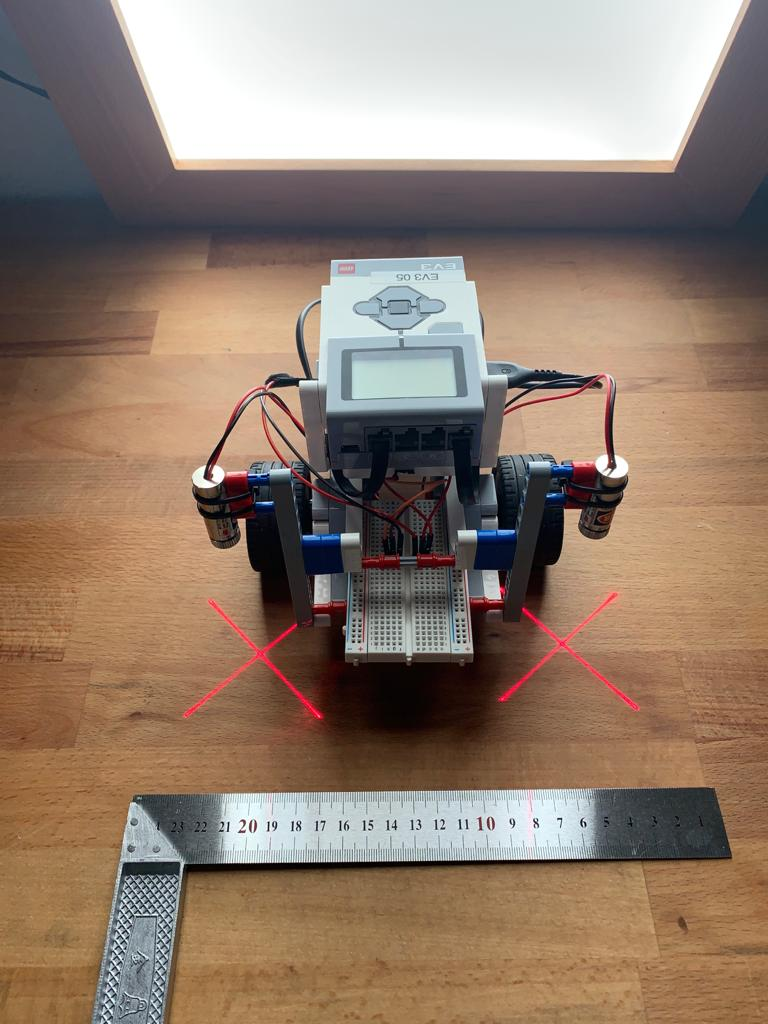
\includegraphics[scale=0.3]{images/FrontView.jpeg}
            \caption{\textcolor{blue}{Rosa - Front View}}
            \label{fig:Rosa front view}
        \end{figure}
        
        \begin{figure}[!ht] %the h places the image nicely if the scale fits
            \centering
            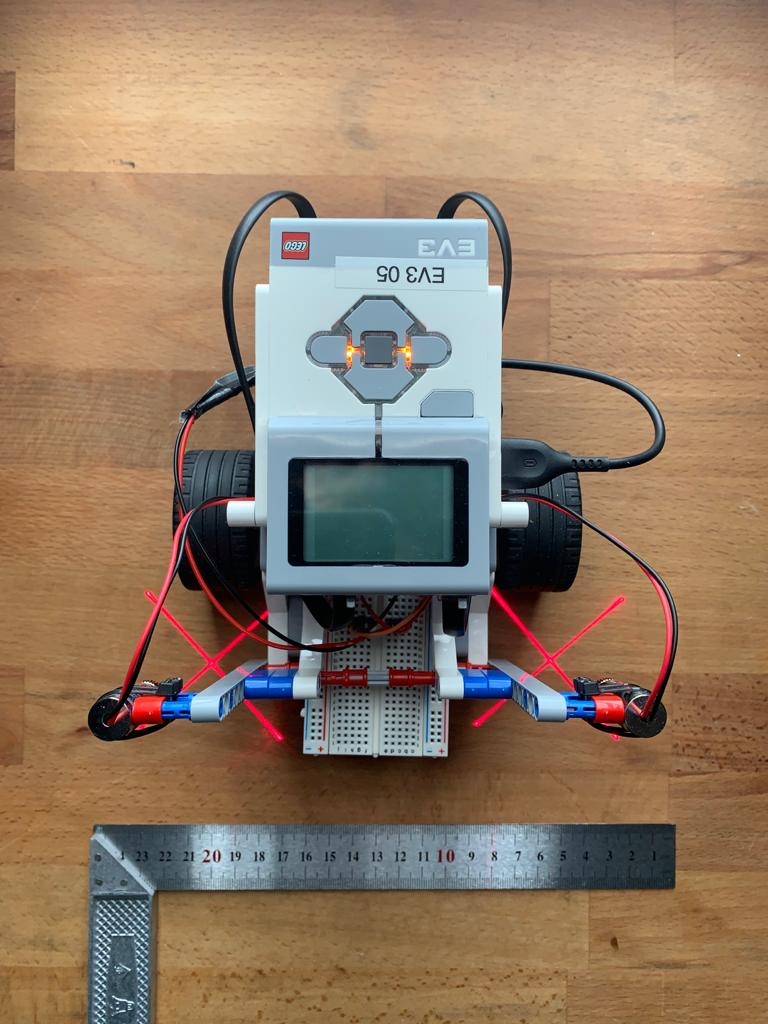
\includegraphics[scale=0.3]{images/TopView3.jpeg}
            \caption{\textcolor{blue}{Rosa - Top View}}
            \label{fig:Rosa top view}
        \end{figure}
        
        \item The following are the materials used for building Rosa \textcolor{blue}{and hence represents the \textbf{measurement facility}}:
        \begin{itemize}
            
            \item[1.] Lego EV3 kit
            \item[2.] Focusable Laser Module (2 units): \textcolor{blue} {It uses a working voltage of 3.0 - 5.0 V. It is powered from the USB port from the EV3 controller.}
            \item[3.] \textcolor{blue}{Bread Board: for making connections between the laser module and the USB port}
            \item[4.] Jumpers for powering the laser modules
        \end{itemize}
        
        \item The robot is three-wheeled with a differential drive configuration. In this configuration (Figure \ref{fig:Rosa Side View}, \ref{fig:Rosa Side View 2}), two of the wheels placed in front of the robot on either sides, have independent actuators. The last wheel in the back, is a castor wheel which is non-driven placed for increasing the stability of the bot.
        
        \begin{figure}[!ht] %the h places the image nicely if the scale fits
            \centering
            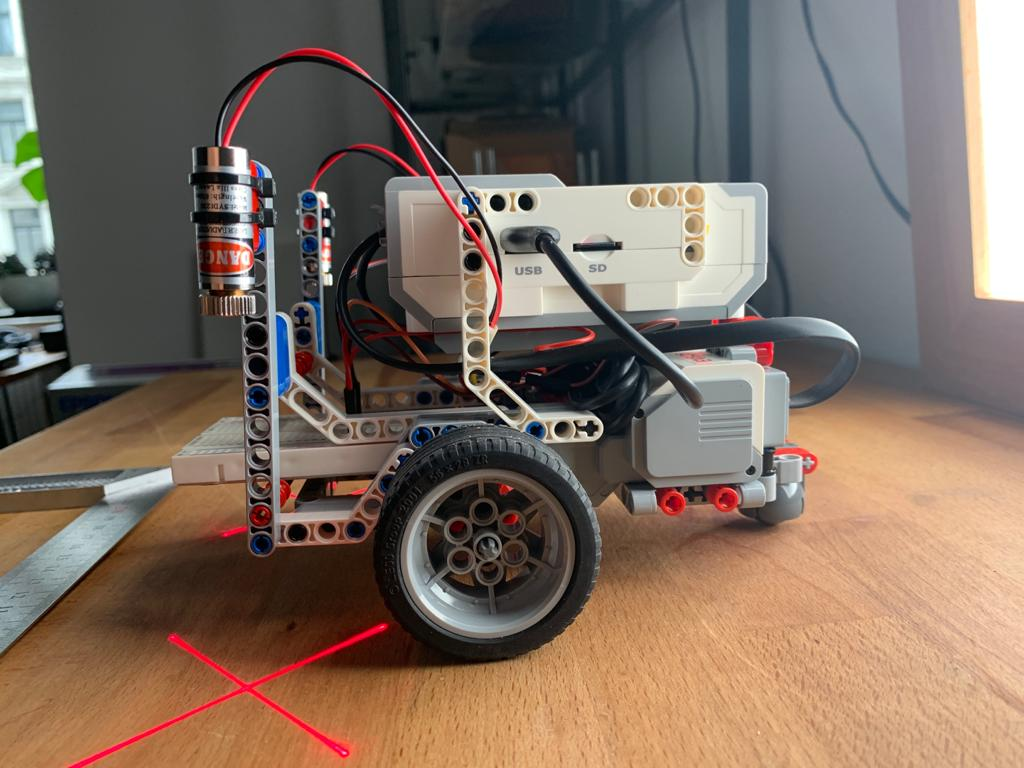
\includegraphics[scale=0.3]{images/SideView.jpeg}
            \caption{\textcolor{blue}{Rosa - Side View}}
            \label{fig:Rosa Side View}
        \end{figure}
        
        \begin{figure}[!ht] %the h places the image nicely if the scale fits
            \centering
            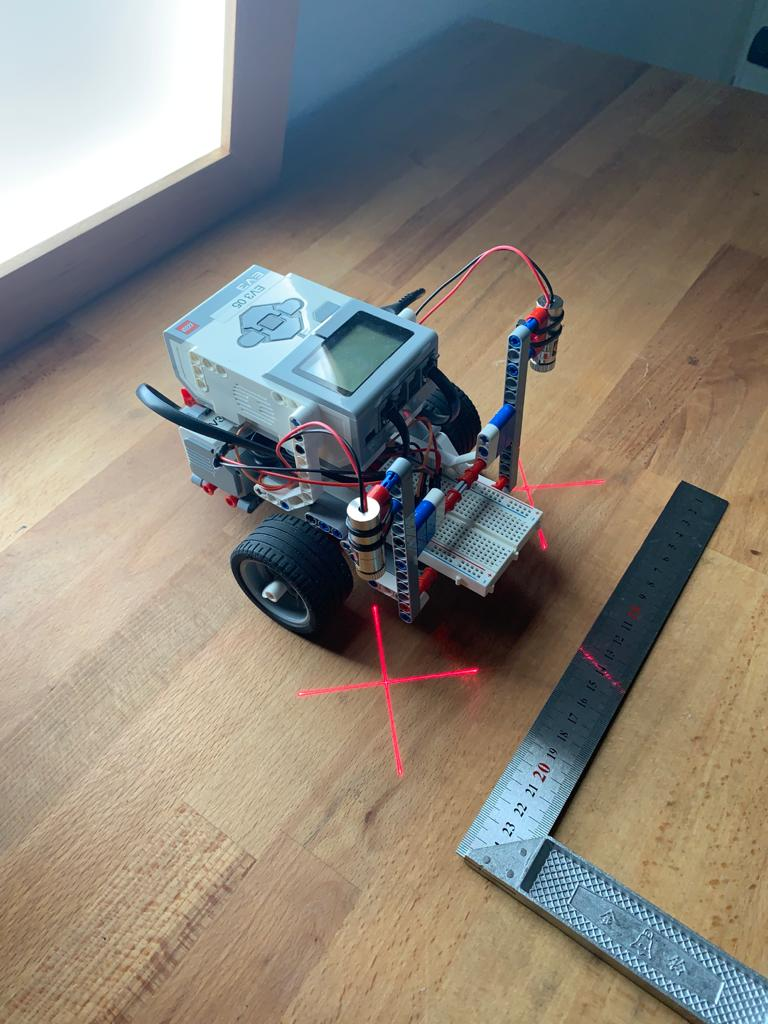
\includegraphics[scale=0.3]{images/SideView2.jpeg}
            \caption{\textcolor{blue}{Rosa - Another Side View}}
            \label{fig:Rosa Side View 2}
        \end{figure}
        
        \item Commands for forward, right and left motions are made from the EV3 controller which is placed on top of the base of the bot.
        
        \item The measurements of the bot's motions are made on top a \textcolor{blue}{96.8 $\times$ 68 cm} sized grid sheet (grid size $\approx 2.5$ cm). 
        
        \begin{figure}[!ht] %the h places the image nicely if the scale fits
            \centering
            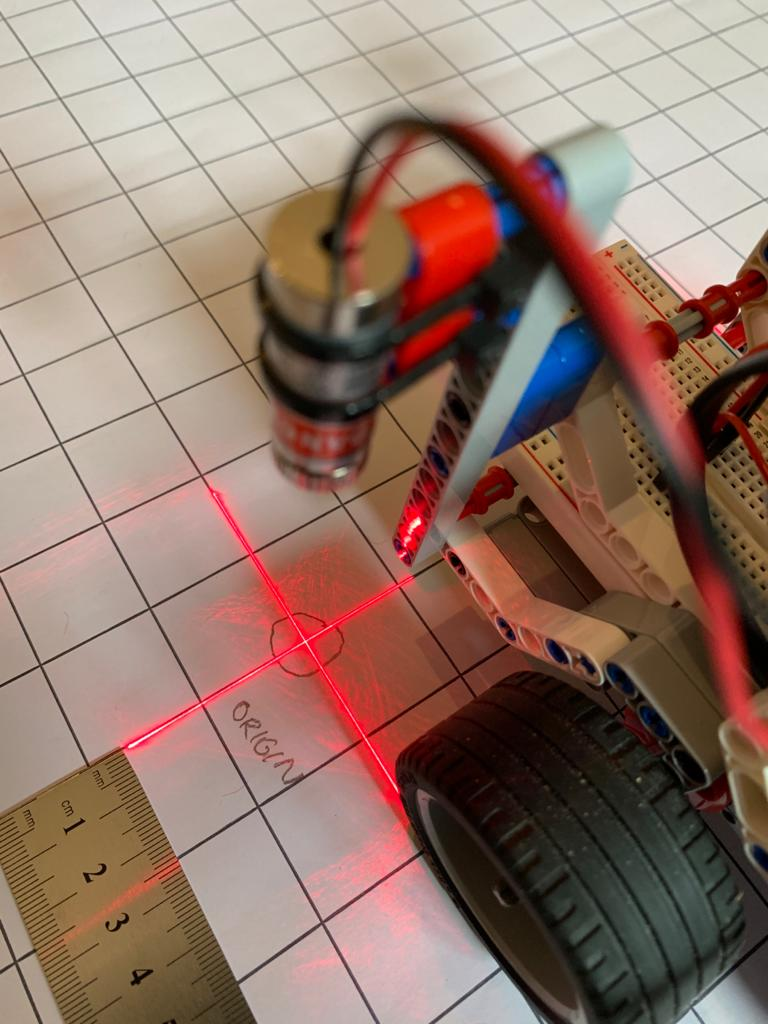
\includegraphics[scale=0.3]{images/Measurement Facility.jpeg}
            \caption{\textcolor{blue}{Rosa on the grid sheet}}
            \label{fig:Method of measuring grid}
        \end{figure}
        
        \begin{figure}[!ht] %the h places the image nicely if the scale fits
            \centering
            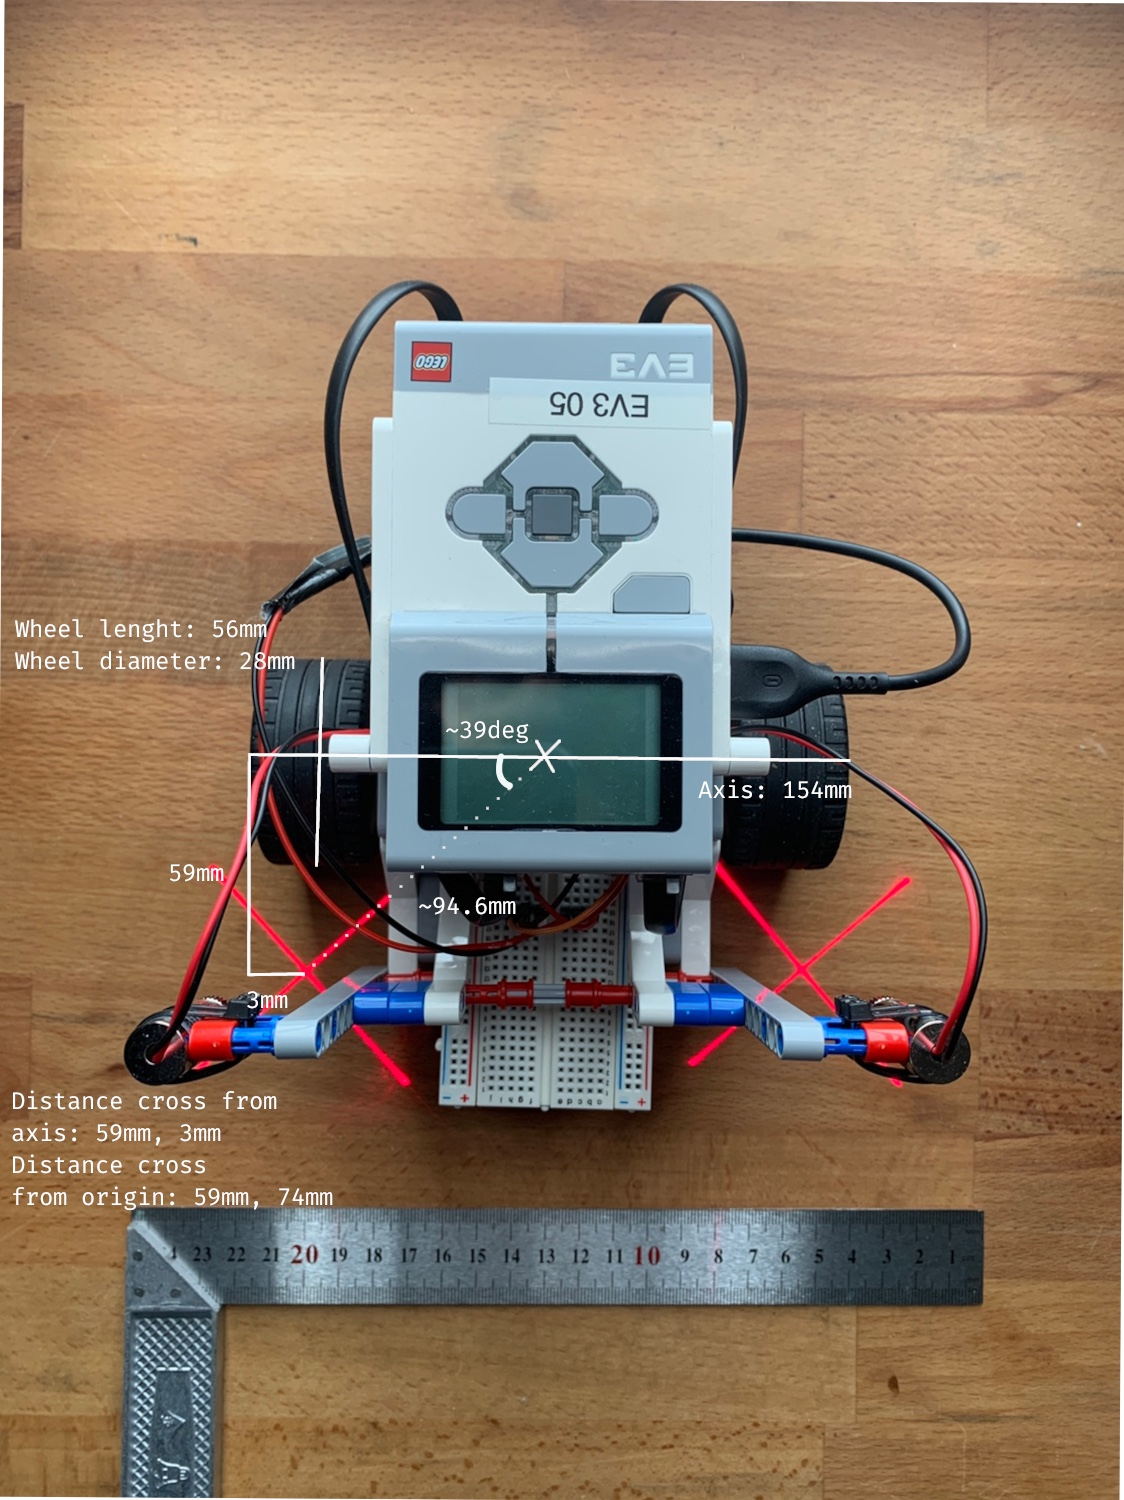
\includegraphics[scale=.30]{images/angle.jpg}
            \caption{\textcolor{blue}{Rosa with the measurement facility}}
            \label{fig:Method of measuring}
        \end{figure}
        
        \begin{figure}[!ht] %the h places the image nicely if the scale fits
            \centering
            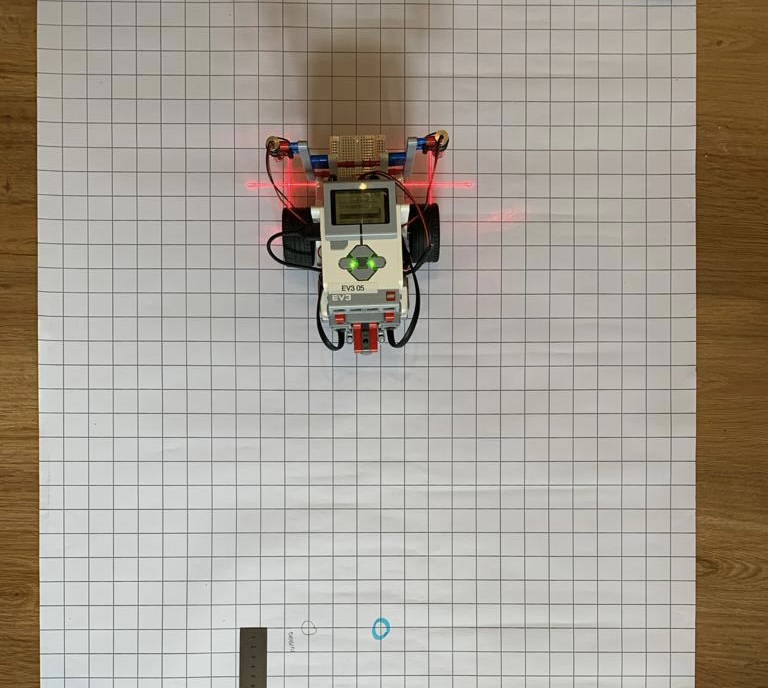
\includegraphics[scale=.60]{images/grid.jpg}
            \caption{\textcolor{blue}{Rosa with the measurement facility 2}}
            \label{fig:Method of measuring 2}
        \end{figure}
        
        
        
        \item The measurement is done by using two focussable \textbf{laser modules} with a resolution of 1mm placed in the front of the robot. \textcolor{blue}{The lasers are mounted onto the lego blocks by using zip ties and tape.}
        
        \item The two cross lasers provide precise marking of the pose of the robot. The aperture is 9.1 cm above ground, and 5.9 cm in front of the main axis. The distance between the two lasers is 14.8 cm. 
        
        \item Since the lasers are working with 5V we are able to use the robots USB port for power supply, which makes any additional batteries unnecessary. \textcolor{blue}{We use a breadboard for making connections between the laser module and the USB port}.
        
        \item The \textbf{pose} of the robot, \textcolor{blue}{which is the \textbf{device under test (DUT)}}, is described by the vector $[x, y, \theta]^T$.
        
        \item \textcolor{blue}{Here, the \textbf{measurand} is $[x, y]^T$ and it represents the \textbf{translation} of the robot which is measured in \textbf{millimeters}. The angle, $\theta$ represents the robot's \textbf{orientation} which is the \textbf{measurement result} obtained from the measured translation, in \textbf{degrees}.}

        \item The Figure \ref{fig:Method of measuring}, \ref{fig:Method of measuring 2} represents the distances between the two cross lasers and the center of the robot. 

        
        % ADD FIGURE
        
        \item Further explanations about the measurement facility is provided in section 1.3 Measurement Process
        
        \item \textbf{Ensuring identical start positions}:
        \begin{itemize}
            \item[1.] Securing the \textcolor{blue}{96.8 $\times$ 68 cm sized} grid sheet to a wooden plank with tape to prevent errors from changes in it's position. % ADD FIGURE
            \item[2.] Marking the start points with the help of laser crosses of the resolution 1mm.
        \end{itemize}
        
        \item \textbf{{Marking stop positions}}:
        \begin{itemize}
            \item[1.] The stop positions are marked with the help of the laser crosses, rulers and pencils on the grid. \textcolor{blue}{The mid point of the laser cross is marked with a pencil and the distance between the starting and end positions are measured using  a ruler.}
            % ADD FIGURE
        \end{itemize}
    \end{itemize}
    
    }
    
    \section{Measurement Process}
        \begin{itemize}
            \item The cross lasers allow us to mark easily positions on the supplied grid paper.
            
            \begin{itemize}
                \item [1.]	
            The robot gets put onto the start position. For this we are using the lasers to position the robot exactly on its start position marks. For a faster positioning, we use a wooden plank on the back of the start position for guidance. 
            \item [2.] We start the robot's program and let it run.
            \item [3.] Using a ruler we make small cross marks at both laser positions. Each cross marks get a number for later data survey.
            \item [4.] The process (2 and 3) is repeated until enough data is gathered.
            \item [5.] Now the cross marks needs to be measured. \textcolor{red}{For this, we use a two step measurement process. We count the number of grids until the grid with the marked cross. Then, }\textcolor{blue}{the mid point of the laser cross is marked with a pencil and the distance between the starting and end positions are measured using  a ruler.}
            \item[6.] \textcolor{blue}{Each measurement is made by keeping in reference, the global coordinate system which is positioned at the centre of the axis connecting the wheel base.}
            \end{itemize}
            
            \item  We define the coordinate system of the robot as following: 
            \item The origin of the robot will lie on the mid point of the axial line connecting the wheels as seen on Figure \ref{fig:Dimensions of the robot} 
            
            \begin{figure}[!ht] 
                        \centering 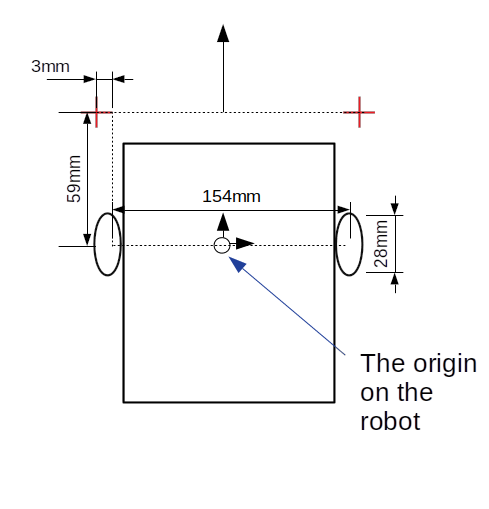
\includegraphics[scale=0.5]{"images/robot_dimensions.png}
                        \caption{Dimensions of the robot}
                        \label{fig:Dimensions of the robot}
                 \end{figure}
            
            
            \item The start position will always be set by aligning the left laser marker on a pre-marked position on the grid. The global coordinate system will also originate from this point, even when measuring the laser crosses for translation and orientation change.
            
            \item \textcolor{blue}{The global coordinate system originate at the initial position of the mid point of the axis connecting the robot's wheels(initial position of the robot's origin). Since the magnitude change of x and y ($\Delta x$  \& $\Delta y$) will be the approximately same for the two markers and the origin of the robot, to take the distance travelled by the robot origin we take the average change in $x$ and $y$ of the two markers. This distance will also be the x and y values with respect to the global coordinate system. The change in orientation will be found using the direction vector connecting the front and rear markers .  See Figure \ref{fig:Robot orientation} and equation \ref{Angle calculation} for details.} 
            
            
            \begin{figure}[!ht] 
                        \centering 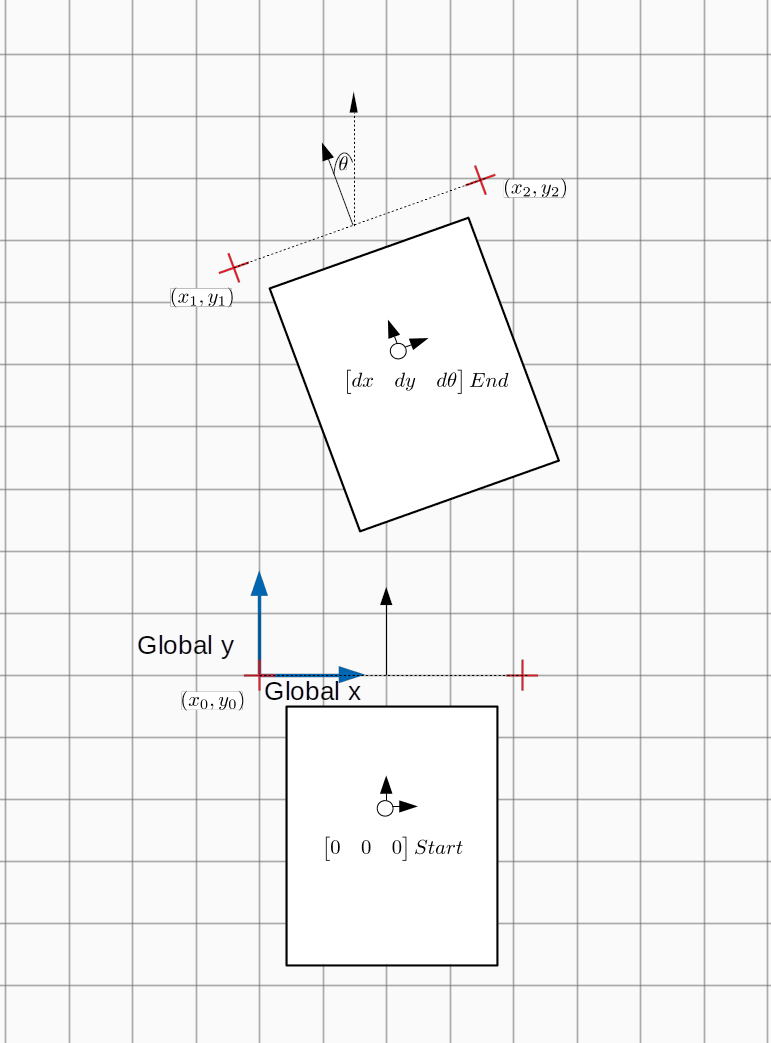
\includegraphics[scale=0.3]{"images/robot_orientation2.png}
                        \caption{Robot orientation}
                        \label{fig:Robot orientation}
                 \end{figure}
            
            
        \end{itemize}
        
        
                
    
    {
    \subsection{Estimate of Error}
    
        \begin{itemize}
            \item The robot's distance measurements will be subjected to many errors. Some of them are listed below along with the rough estimate of their precision:
            
            \begin{itemize}
                \item[1.] Error when marking the laser cross \textcolor{blue}{due to the thickness of the laser crosses:}  $\pm 2mm$
                
                \item[2.] Parallax error when measuring the laser cross with the ruler \textcolor{blue}{used for our measurements:} $\pm 1mm$
                
                \item[3.] Pressing the button pushes the robot from one position and can put extra weight on one side of the wheel\textcolor{blue}{:} $\pm \textcolor{blue}{4 } mm$
                
                \item[4.] Slippage: during multiple runs the laser markers can slightly change position\textcolor{blue}{:} $\pm 1mm$
                
                \item[5.] If the grid is not held tightly there will be folds and the surface will not be flat\textcolor{blue}{:} $\pm 1mm$
                
                \item[6.] Jerk: The sudden deceleration of the robot can overshoot the robot past its position specially if the momentum of the controller. This will not be same in every run.\textcolor{blue}{:} $\pm 2mm$ \textcolor{blue}{(not a measurement error)}
            \end{itemize}
            
        \end{itemize}
    
    
    
    
    
    }
    
    \section{Error Propagation}
    {
        \begin{itemize}
            \item The errors mentioned above will propagate when making the distance measurements. This can be easily calculated using a Jacobian.
            
            \item Since there are 4 variables namely $x_1,x_2,y_1,y_2$ (refer Figure \ref{fig:Robot orientation} for naming convention), the error associated to each of them contribute to the propagated error.
            
            \item The orientation is given by the equation \ref{Angle calculation}. \textcolor{blue}{Since in our design the laser pointers are aligned along the x axis instead of the y axis the we calculate  $\frac{\pi}{2}-\theta$ instead of directly finding $\theta$ therefore the orientation finding equation is slightly modified as below:}
            \begin{equation}\label{Angle calculation}
                \textcolor{red}{\frac{\pi}{2}-\theta=\tan^{-1}(\frac{y_2-y_1}{x_2-x_1})}
            \end{equation}
            
            \item If the variable matrix is defined as:
            \begin{equation}\label{Variable Matrix}
                \begin{bmatrix}x_{1}\\x_{2}\\y_{1}\\y_{2}\end{bmatrix}
            \end{equation}
            
            \item Then the Jacobian will be:
          
            
            
           $$ \begin{bmatrix}\label{Jacobian}- \frac{y_{1} - y_{2}}{\left(- x_{1} + x_{2}\right)^{2} + \left(- y_{1} + y_{2}\right)^{2}} & \frac{y_{1} - y_{2}}{\left(- x_{1} + x_{2}\right)^{2} + \left(- y_{1} + y_{2}\right)^{2}} & - \frac{- x_{1} + x_{2}}{\left(- x_{1} + x_{2}\right)^{2} + \left(- y_{1} + y_{2}\right)^{2}} & \frac{- x_{1} + x_{2}}{\left(- x_{1} + x_{2}\right)^{2} + \left(- y_{1} + y_{2}\right)^{2}}\end{bmatrix}
           $$
           
           
            
               
          \item The upper bound and lower bound of errors were defined according to Figure \ref{fig:Error Bounds} . The green arrows represent the vector in which direction the error should propagate for it to be the upper or lower bounds of the error.    
          
          \begin{figure}[ht!] 
                        \centering
                        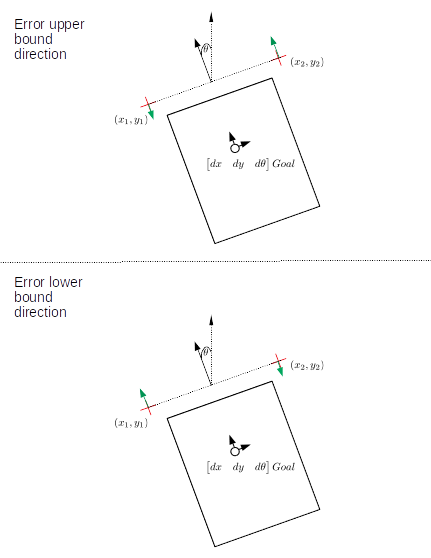
\includegraphics[scale=0.8]{"images/error_propagation_direction.png}
                        \caption{\textcolor{red}{Error Bounds}}
                        \label{fig:Error Bounds}
         \end{figure}
                
                
            
        \item The python code given below is used to calculate the propagated error. In order to demonstrate the propagation of error, 5 runs of the straight, left and right motions were carried out. 
        
        \item Note that for this example we used \textbf{only} the parallax error of measuring the laser cross with the ruler, with an estimated error of $\pm$1mm. Therefore, the upper bound the error values will be $[0.1, -0.1, -0.1, 0.1]$ (in centimeters) and the lower bound will be $[-0.1, 0.1, 0.1, -0.1]$ (in centimeters); where the variables are in the order of $[dx_1, dx_2, dy_1, dy_2]$.
        
        \item \textcolor{red}{The figure \ref{fig:Error Bounds} represent how we arrived at the order for the variables for the lower and upper bound error. We define the error vectors which will account for the direction and the magnitude of the error. }
        
        \item Example:
        
        \item[1.] For straight motion of measurements in order [x1,x2,y1,y2] [ 1.5 16.3 48.1 47.4]
        
        \begin{itemize}
            \item[a.] The error upper bound for straight motion is \textcolor{red}{0.7 \textdegree}
            \item[b.] The error lower bound for straight motion is \textcolor{red}{-0.7 \textdegree}
        \end{itemize}
        
        \item[2.] For left motion of measurements in order [x1,x2,y1,y2] [-19.3 -11.2  24.6  36.8]
        
        \begin{itemize}
            \item[a.] The error upper bound for left motion is \textcolor{red}{1.1 \textdegree} 
            \item[b.] The error lower bound for left motion is \textcolor{red}{-1.1 \textdegree }
        \end{itemize}

        \item[3.] For right motion of measurements in order [x1,x2,y1,y2] [27.4 35.3 37.1 24.5]
        
        \begin{itemize}
            \item[a.] The error upper bound for right motion is \textcolor{red}{-0.3 \textdegree }
            \item[b.] The error lower bound for right motion is \textcolor{red}{0.3 \textdegree }
        \end{itemize}


            
        \begin{minted}{python}
    import numpy as np
    import sympy as sp
    import os
    import sys
    
    ## All distances measurement are in centimeters(cm) and angles in radians 


def error_upper_bound(lamd_jacobian, lamd_theta_eq, 
                      coordinate_list, error_model=[0.1,-0.1,-0.1,0.1]):
    
    '''
    Calculate the upper error bound
    
    Parameters
    ----------------
    lamd_jacobian  : A lamdified jacobian matrix acting like a numpy array
    lamd_theta_eq  : A lamdified variable matrix acting like a numpy array
    coordinate_list: The current coordinates of the robot
    error_model    : The estimated error bounds for robot
    
    
    Returns
    ----------------
    A numpy array of propagated upper bound error
    
    
    '''
    
    ## The variables are in the order x1, x2, y1, y2
    current_jacobian = lamd_jacobian(coordinate_list[0], coordinate_list[1],
                                     coordinate_list[2], coordinate_list[3])
    current_theta_eq = lamd_theta_eq(error_model[0], error_model[1], 
                                     error_model[2], error_model[3])
    
    return np.dot(current_jacobian, current_theta_eq)
    


def error_lower_bound(lamd_jacobian, lamd_theta_eq, 
                      coordinate_list, error_model=[-0.1,0.1,0.1,-0.1]):
    '''
    Calculate the lower error bound
    
    Parameters
    ----------------
    lamd_jacobian  : A lamdified jacobian matrix acting like a numpy array
    lamd_theta_eq  : A lamdified variable matrix acting like a numpy array
    coordinate_list: The current coordinates of the robot
    error_model    : The estimated error bounds for robot
    
    
    Returns
    ----------------
    A numpy array of propagted lower bound error
    
    
    '''
    ## The variables are in the order x1, x2, y1, y2
    current_jacobian = lamd_jacobian(coordinate_list[0], coordinate_list[1],
                                     coordinate_list[2], coordinate_list[3])
    current_theta_eq = lamd_theta_eq(error_model[0], error_model[1],
                                     error_model[2], error_model[3])
   

    return np.dot(current_jacobian, current_theta_eq)
    
## Create the jacobian for the matrix
## Even if the angle theta is 90-calulated angle the error propagation is the same 

## Creating the Jacobian

x1,x2,y1,y2,theta = sp.symbols('x1,x2,y1,y2,theta')

## Check here if it should be atan or atan2. Using sp.arctan2 as per
## comments recevied during peer-review
eq1 = sp.arctan2((y2-y1),(x2-x1))

theta_eq = sp.Matrix([eq1])
measurement_eq = sp.Matrix([x1, x2, y1, y2])

error_jacobian = theta_eq.jacobian(measurement_eq)
print("The Jacobian is \n")
display(error_jacobian)

print(f"The error matrix is \n")
display(measurement_eq)

print("\n \n The error function is \n ")
display(error_jacobian*measurement_eq)
lamd_jacobian = sp.lambdify([x1, x2, y1, y2], error_jacobian,'numpy')
lamd_theta_eq = sp.lambdify([x1, x2, y1, y2], measurement_eq,'numpy')

##This is a test run data from 5 runs in each category(straigh,left and right)
## This dictionary is here to easily show how the data was collected 
## A sepearate list will be made to make this calling of data easier
sample_test_data_1={
    "straight": [
        {"x1": 1.5, "y1": 48.1, "x2": 16.3, "y2": 47.4},
        {"x1": -1.5, "y1": 46.9, "x2": 13.2, "y2": 47.3},
        {"x1": -3.1, "y1": 45.5, "x2": 14.2, "y2": 46.4},
        {"x1": 0.7, "y1": 45.1, "x2": 15.4, "y2": 44.7},
        {"x1": -0.2, "y1": 45.8, "x2": 14.7, "y2": 45.9}
    ],
    "left": [
        {"x1": -19.3, "y1": 24.6, "x2": -11.2, "y2": 36.8},
        {"x1": -20.1, "y1": 26.5, "x2": -12.1, "y2": 39.0},
        {"x1": -19.8, "y1": 26.8, "x2": -11.7, "y2": 39.2},
        {"x1": -21.1, "y1": 24.9, "x2": -13.4, "y2": 37.5},
        {"x1": -18.6, "y1": 25.6, "x2": -10.0, "y2": 37.6}
    ],
    "right": [
        {"x1": 27.4, "y1": 37.1, "x2": 35.3, "y2": 24.5},
        {"x1": 28.1, "y1": 36.9, "x2": 35.7, "y2": 24.1},
        {"x1": 27.8, "y1": 39.1, "x2": 35.6, "y2": 26.4},
        {"x1": 27.1, "y1": 38.1, "x2": 35.0, "y2": 25.6},
        {"x1": 27.6, "y1": 39.2, "x2": 35.1, "y2": 26.7}
    ],
    "origin": {"x0": 0, "y0": 0, "x0_2": 14.8, "y0_2": 0}
}

def call_data(cat,index):
    '''
    This functions retuns the values from the dictionary of sample run data
    Parameters
    ------------------------
    cat   : The category of motion eg:Left -> char
    index : The index of run               -> int
    
    Returns
    ------------------------
    out_list: output the list of data in order [x1,x2,y1,y2] -> list
    
    
    '''
    
    if cat=='s':
        out_list = np.array([sample_test_data_1['straight'][index]['x1'],
                             sample_test_data_1['straight'][index]['x2'],
                             sample_test_data_1['straight'][index]['y1'],
                             sample_test_data_1['straight'][index]['y2']])
        
    if cat=='l':
        out_list = np.array([sample_test_data_1['left'][index]['x1'],
                             sample_test_data_1['left'][index]['x2'],
                             sample_test_data_1['left'][index]['y1'],
                             sample_test_data_1['left'][index]['y2']])
        
    if cat=='r':
        out_list=np.array([sample_test_data_1['right'][index]['x1'],
                           sample_test_data_1['right'][index]['x2'],
                           sample_test_data_1['right'][index]['y1'],
                           sample_test_data_1['right'][index]['y2']])
    
    
    return out_list
    
    
    ## Use this line to manually enter for a error bound



## The variables are in the order x1, x2, y1, y2


coordinate_list = call_data('s', 0)
error_upper_straight = error_upper_bound(lamd_jacobian,lamd_theta_eq, coordinate_list)
error_lower_straight = error_lower_bound(lamd_jacobian, lamd_theta_eq, coordinate_list)


coordinate_list=call_data('l',0)
error_upper_left=error_upper_bound(lamd_jacobian,lamd_theta_eq,coordinate_list)
error_lower_left=error_lower_bound(lamd_jacobian,lamd_theta_eq,coordinate_list)


coordinate_list = call_data('r', 0)
error_upper_right = error_upper_bound(lamd_jacobian,lamd_theta_eq, coordinate_list)
error_lower_right = error_lower_bound(lamd_jacobian, lamd_theta_eq, coordinate_list)


print(f'The error upper bound for straight motion is {error_upper_straight[0][0]} radians \n')
print(f'The error lower bound for straight motion is {error_lower_straight[0][0]} radians \n')

print(f'The error upper bound for left motion is {error_upper_left[0][0]} radians \n')
print(f'The error lower bound for left motion is {error_lower_left[0][0]} radians \n')

print(f'The error upper bound for right motion is {error_upper_right[0][0]} radians \n')
print(f'The error lower bound for right motion is {error_lower_right[0][0]} radians \n')


##Use this to read from text file of the positions and calculate error for each reading

file_path = os.path.join(os.getcwd(),'coordinate_list.txt')
with open(file_path) as file:
    data = file.readlines()


propagated_error=np.zeros((len(data),6))

file_name='Propagated_Error'
try:


    f=open(file_path+file_name,'x') ##Open/Create a file to store data


except :

    print("\n Maps already exist in results folder \n")



for position in data:
    
    error_upper=error_upper_bound(lamd_jacobian,lamd_theta_eq,position)
    error_lower=error_lower_bound(lamd_jacobian,lamd_theta_eq,position)
    propagated_error[0:3]=position
    propagated_error[4]=error_upper
    propagated_error[5]=error_lower
    f.write(propagated_error+'\n')
    
    
f.close()
    
    

    

        
    
    
    
    
    \end{minted}    
            
            
        \end{itemize}
    }
    
    
\end{document}
